\documentclass[10pt,a4paper]{article}
%\usepackage[english,spanish]{babel}
\usepackage{indentfirst}
\usepackage{anysize} % Soporte para el comando \marginsize
%\marginsize{1.5cm}{1.5cm}{0.5cm}{1cm}
\marginsize{2,5cm}{1,8cm}{4cm}{1,7cm}
\usepackage[psamsfonts]{amssymb}
\usepackage{amssymb}
\usepackage{amsfonts}
\usepackage{amsmath}
\usepackage{amsthm}
\usepackage{stackrel}
\usepackage{graphicx}
\usepackage[colorinlistoftodos]{todonotes}
%Color a las referencias
\usepackage[colorlinks=true, allcolors=blue]{hyperref}
\usepackage[spanish]{babel}
\selectlanguage{spanish}
\usepackage[utf8]{inputenc} 

\usepackage{multicol}
\renewcommand{\thepage}{}
\columnsep=7mm

%%%%%%%%%%%%%%%%%%%%%%%%%%%%%%%%%%%%%%%%
\newtheorem{definicion}{Definici\'on}[section]
\newtheorem{teorema}{Teorema}[section]
\newtheorem{prueba}{Prueba}[section]
\newtheorem{prueba*}{Prueba}[section]
\newtheorem{corolario}{Corolario}[section]
\newtheorem{observacion}{Observaci\'on}[section]
\newtheorem{lema}{Lema}[section]
\newtheorem{ejemplo}{Ejemplo}[section]
\newtheorem{solucion*}{Soluci\'on}[section]
\newtheorem{algoritmo}{Algoritmo}[section]
\newtheorem{proposicion}{Proposici\'on}[section]

\linespread{1.4} \sloppy

\newcommand{\R}{\mathbf{R}}
\newcommand{\N}{\mathbf{N}}
\newcommand{\C}{\mathbb{C}}
\newcommand{\Lr}{\mathcal{L}}
\newcommand{\fc}{\displaystyle\frac}
\newcommand{\ds}{\displaystyle}

\DeclareMathOperator{\Dom}{Dom}

%%%%%%%%%%%%%%%%%%%%%%%%%%%%%%%%%%%%%%%%

\renewcommand{\thefootnote}{\fnsymbol{footnote}}
\usepackage{url}
\usepackage{hyperref}
\begin{document}
\begin{center}
 {\Large \textbf{MODELAMIENTO DE LA ECONOMÍA DE UN PAÍS}}
\end{center}
\begin{center}
 Gustavo Lozano$^{1}$, Miller Silva$^{2}$, Victor Ponce$^{3}$, Kevin Solano$^{4}$, Nicks Lazaro$^{5}$ elazaroc@uni.pe , \vskip5pt
 
{\it Facultad de Ciencias, Universidad Nacional de Ingenier\'{\i}a\\}
\end{center}
%\maketitle 
\vspace*{1cm}
\begin{abstract}

\noindent Las matemáticas son de gran importancia y ayuda para el progreso de muchas disciplinas, como por ejemplo la economía. El desarrollo de este método combina el uso de la teoría económica, el análisis estadístico y matemático. Introducir ciertas simplificaciones y supuestos para crear un modelo que ayudara a predecir los niveles de producción futuros de cada sector o industria, a fin de satisfacer las demandas futuras para diversos productos. La actividad económica en la región se divide en un número de segmentos o de sectores productivos. Cada sector agrupa actividades que tienen diferentes ritmos de consumo y producción de bienes. Parte de la producción de un sector (Output) puede ir al consumo (Input) de otro distinto sector. Esta información se recolecta en forma de una matriz. Los paises poseen muchas industrias relevantes causando que se generan matrices muy grandes, encontrar la solucion manualmente es muy ineficiente, por ello recurimos al uso de computadores. Para poder confiar en los resultados de la maquina hacemos uso del \textbf{análisis numérico} encontrando los metodos adecuados para obtener la solución con menor error.

\end{abstract}

\begin{quotation}
	{\small
		\noindent\textbf{Palabras Clave:} \\ 
	Análisis estadístico, Demanda futura, Sector industrial, Producción futura, Análisis numérico\\
	}
\end{quotation}

\renewcommand{\abstractname}{Abstract}
\begin{abstract}
	\noindent Mathematics is of great importance and helps the progress of many disciplines, such as economics. The development of this method combines the use of economic theory, statistical and mathematical analysis. Economic activity in the region is divided into a number of segments or productive sectors. Each sector groups activities that have different rates of consumption and production of goods. Part of the production of a sector (Output) can go to the consumption (Input) of another different sector. This information is collected in the form of a matrix. Countries have a large number of industries, which generates very large matrices, finding the solution manually is very inefficient, therefore, we resort to the use of computers. To be able to trust the results of the machine, we make use of the \textbf{Numerical Analysis} finding the adequate methods to obtain the solution with less error.
	
\end{abstract}


\begin{quotation}
	{\small
		\noindent \textbf{Keywords:} \\ 
		Statistical analysis, Future demand, Industrial sector, Future production, Numerical analysis\\
	}
\end{quotation}


\pagebreak

\begin{multicols}{2}
\begin{center}
{\large \bf 1. INTRODUCCI\'ON}
\end{center}
 Con el fin de comprender y ser capaz de manipular la economía de un país o una región, uno tiene que llegar a un cierto modelo basado en los diversos sectores de esta economía. El modelo de Leontief es un intento en esta dirección. Basado en la suposición de que cada industria en la economía tiene dos tipos de exigencias: la demanda externa (de fuera del sistema) y la demanda interna (demanda de una industria por otro en el mismo sistema), el modelo de Leontief representa la economía como un sistema de ecuaciones lineales. El modelo de Leontief fue inventado en los años 30 por el profesor Wassily Leontief \color{blue} Fig 1 \color{black} que desarrolló un modelo económico de la economía de Estados Unidos mediante su división en 500 sectores económicos. El 18 de octubre de 1973, el profesor Leontief fue galardonado con el Premio Nobel de economía por su esfuerzo.\\
 
\begin{center}
	
	
	\centering
	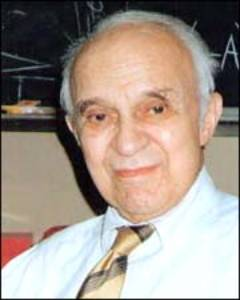
\includegraphics[width=5cm,height=5cm]{leontief.jpg}
	\\
	Fig1: Profesor Wassily Leontief
\end{center}

\begin{center}
{\large \bf 2. CONCEPTOS PREVIOS}
\end{center}
Hay dos tipos de modelados de la economía que estableció Leontief: el modelo cerrado y el modelo abierto.\\
\begin{itemize}
	\item \textbf{EL MODELO CERRADO DE LEONTIEF} : Considerar una economía que consiste en $n$ industrias (o sectores)   $S_{1}, ... , S_{n}$. Eso significa que cada industria consume algunos de los bienes producidos por las otras industrias, incluso a sí misma (por ejemplo, una planta generadora de energía utiliza parte de su propia energía para la producción). Decimos que tal economía esta cerrada si satisface sus propias necesidades. Es decir, no hay mercancías que salgan o entren en el sistema. Sea $m_{ij}$ el número de unidades producidas por la industria $S_{i}$ y necesarias para producir una unidad de la industria $S_{j}$. Si $p_{k}$ es el nivel de producción de la industria $S_{k}$, luego $m_{ij}p_{j}$ representa el número de unidades producidas por la industria $S_{i}$ y consumidas por la industria $S_{j}$. Entonces, el número total de unidades producidas por la industria $S_{i}$ viene dado por:
\[  p_{1}m_{i1} + p_{2}m_{i2} + ... + p_{n}m_{in} \]
Para tener una economía equilibrada, la producción total de cada industria debe ser igual a su consumo total. Esto nos dará el siguiente sistema lineal:

\begin{equation*}
	\begin{matrix}
	m_{11}p_{1} &+& m_{12}p_{2} &+& \ldots  &+ &m_{1n}p_{n} &=& p_{1}\\
	m_{21}p_{1} &+& m_{22}p_{2} &+&\ldots  &+& m_{2n}p_{n} &=& p_{2}\\
	\vdots&&\vdots&&&&\vdots&&\vdots\\         
	m_{n1}p_{1} &+& m_{n2}p_{2} &+& ... & +& m_{nn}p_{n} &=& p_{n}
	\end{matrix}
\end{equation*}\\
Luego, nuestro sistema lineal será:       
 
 \[ A =
 \left( \begin{array}{cccc}
 m_{11} & m_{12} & \cdots & m_{1n} \\ 
 m_{21} & m_{22} & \cdots & m_{2n} \\
 \vdots & \vdots & \ddots & \vdots \\
 m_{n1} & m_{n2} & \cdots & m_{nn}
 \end{array} \right) \]\\
 
Entonces nuestro sistema a resolver se puede escribir como $AP = P$, donde:
	
 \[ P =
\left( \begin{array}{cccc}
p_{1} \\ 
p_{2} \\ 
\vdots  \\
p_{n} \\ 
\end{array} \right) \]\\
 $A$ es denominada MATRIZ DE ENTRADA-SALIDA.\\
 Luego estamos buscando un vector P que satisfaga $AP = P$ y con componentes no negativos, al menos uno de los cuales sea positivo.\\
 
 \item{\textbf{EL MODELO ABIERTO DE LEONTIEF: }}El primer modelo de Leontief trata el caso en el que no hay mercancías que ingresen a la economia, pero en realidad esto no sucede muy a menudo. Por lo general, una determinada economía tiene que satisfacer una demanda externa, por ejemplo, de organismos como los organismos gubernamentales. En este caso, sea $d_{i}$ la demanda de la industria exterior $Si$, $p_{i}$ y $m_{ij}$ se definen como en el modelo cerrado. Luego tendremos lo siguiente:
 $$ p_{i} = m_{i1}p_{1} + m_{i2}p_{2} + ... + m_{in}p_{n} + d_{i}$$
 para cada $i=1,2,...,n$. Esto nos da el siguiente sistema lineal:  $P = AP + d$, donde $P$ y $A$ son definidos como en el modelo cerrado y $d$ es el vector de demanda:\\
 	\[ d =
 	\left( \begin{array}{cccc}
 	d_{1} \\
 	d_{2} \\ 
 	\vdots  \\
 	d_{n} \\ 
 	\end{array} \right) \]\\
 	
 La manera de obtener nuestro sistema lineal es:
 	$$ P = AP +d \Rightarrow P-AP = d \Rightarrow (I-A)P = d$$
 	el cual sera el sistema a resolver.
 
 Existen varios métodos para resolver un sistema de ecuaciones, pero entre los más conocidos tenemos:
 \begin{itemize}
 	\item \textbf{Método de Gauss:} Consiste en hacer operaciones elementales a la matriz aumentada hasta llevarlo a una triangular superior
 	\begin{equation*}
 		\begin{bmatrix}
	 		a_{11}&a_{12}&a_{13}&\cdots&a_{1n}&|&b_{1}\\
	 		0&a_{22}&a_{23}&\cdots&a_{2n}&|&b_{2}\\
	 		0&0&a_{33}&\cdots&a_{3n}&|&b_{3}\\
	 		\vdots&\vdots&\vdots&\ddots&\vdots&|&\vdots\\
	 		0&0&0&\cdots&a_{nn}&|&b_n
 		\end{bmatrix}
 	\end{equation*}
 	la cual puede ser resuelta hallando los valores de las variables de abajo hacia arriba.
 	\item \textbf{Método Gauss-Jordan:} Dado el sistema $Ax=b$, lo que este método principalmente hace es hallar la inversa de $A$ para luego obtener la solución de la siguiente manera $$x=A^{-1}b$$ 
 	\end{itemize}
\end{itemize}
\newpage
%\vspace*{1cm}
\begin{center}
{\large \bf 3. AN\'ALISIS}
\end{center}
Vamos a trabajar con el modelo abierto ya que este se asemeja más a la realidad. Supongamos que tenemos los datos del comportamiento de un sistema abierto, de 20 industrias (en dólares), en la matriz $A $ y $d$: (click en el siguiente cuadro)

\href{https://nbviewer.jupyter.org/github/MillerSilva/numerical-analysis/blob/master/genera_sistema.ipynb}{Matriz A y d}
\\
\noindent Donde $a_{ij}$ es el dinero con el que $S_j$ compra productos a la industria $S_i$ para producir \$1 de producto y $d_i$ es la demanda exterior que tiene la industria $S_i$.

\noindent Ahora aplicando el modelo abierto de Leontief, nuestro sistema a resolver es $$(I-A)P=d$$ donde $P_i$ es la producción total(en dólares) de la industria $S_i$.
%\begin{center}
%{\large \bf 4. OBSERVACIONES}
%\end{center}
%
%\begin{center}
%{\large \bf 5. CONCLUSIONES}
%\end{center}

%\begin{center}
%{\large \bf Agradecimientos}
%\end{center}
%Los autores agradecen a las autoridades de la Facultad de Ciencias de la Universidad Nacional de 
%Ingenier\'{\i}a por su apoyo.
%%\begin{center}
%%{\large \bf Apendice: }
%%\end{center}

\end{multicols}

%\begin{center}
% -----------------------------------------------------------------------------
%\end{center}
\begin{multicols}{2}
%\begin{list}{}{\setlength{\topsep}{0mm}\setlength{\itemsep}{0mm}%
%\setlength{\parsep}{0mm}\setlength{\leftmargin}{4mm}}
%%
%%------------------------------------- References --------------------
%\small
%\item[1.] I.K. Argyros, \textit{Newton-like methods under mild \linebreak differentiability conditions with error analysis,} Bull. \linebreak Austral. Math. Soc. \textbf{37} (1988), 131-147.
%\item[2.] 
%%---------------------------------------------------------------------
%%
%\end{list}
\end{multicols}
\end{document}%\grid
